\documentclass[10pt,aspectratio=169]{beamer}
% Packages
\usepackage{mathabx}
\usepackage{xcolor}
\usepackage{amsmath}
\usepackage{mathtools}
\usepackage{standalone}
\usepackage{mhchem}
\usepackage{textpos}
\usepackage{graphicx}
\usepackage{wrapfig}
\graphicspath{{images}}

% Configure template
\setbeamertemplate{navigation symbols}{}

% Theme
\usetheme[progressbar=frametitle]{metropolis}
\setbeamertemplate{caption}[numbered]
\setbeamersize{text margin left=5mm,text margin right=5mm}

% Title page details: 
\title{Scientific Computing: Molecular dynamics}
\subtitle{Problemsheet 1}
\author{Jimin Kim, Christian Nix, Noah Schlenker}
\date{03. Mai 2024}
\institute{Technical University of Munich}

\begin{document}

% Title page frame
\maketitle

\addtobeamertemplate{frametitle}{}{
\begin{textblock*}{100mm} (.945\textwidth,-.85cm)

\includegraphics[scale=0.14]{../template/res/tum_logo.png}
\end{textblock*}}

% Outline frame
\begin{frame}{Outline}
    \tableofcontents
\end{frame}

% Slides for mac_setup
\section{Mac Setup}

\begin{frame}
    \frametitle{Using docker to remotelz build the project}

    \textbf{Problem:} xerces is not available on MacOS and code will be evaluated on a Linux system

    \textbf{Solution:} Clion offers remote toolchains to build, run, and debug project

    \begin{itemize}
        \item Similar to WSL described on problem sheet for Windows
        \item Create Docker container with Ubuntu base image and all necessary files and libraries
        \item Create a new toolchain in Clion
        \item Configure Clion's Cmake profile and configuration to use the created docker image
        \item Use the IDE as you normally would
        \item Even connect to the container via terminal to do intensive debugging
    \end{itemize}

    \textbf{Be aware that this approach will have its limits}
\end{frame}

% Slides for mac_setup
\section{Particle container}

\begin{frame}
    \frametitle{Realization of the particle container using vectors}
    \textbf{Task:} Create a class to encapsulate the particles for quick access and convenient iteration

    \textbf{Solution:} Class ParticleContainer

    \begin{itemize}
        \item Storing particles as a std::vector
        \item Iterator functions for convenient particle iteration
        \item Pairwise iterator with only unique pairs
    \end{itemize}
    $\Rightarrow$ Operators for range-based loop conditions (e.g. for (\textbf{begin}; \textbf{end}; \textbf{++};))
\end{frame}

% Slides for mac_setup
\section{Design pattern}

\begin{frame}
    \frametitle{Refactoring with the strategy pattern}
    \textbf{Problem:} Methods for I/O and calculations will change frequently

    \textbf{Solution:} Strategy as the implemented design pattern

    \begin{columns}
        \hspace{-25pt}
        \begin{column}{0.55\textwidth}
            \begin{itemize}
                \item Define a family of algorithms and encapsulate them
                \item \textbf{Structure: } 
                \begin{itemize}
                    \item Simulation as the highest layer for choosing strategy
                    \item Compartmentalizing I/O, model and physics
                    \item Enabling Combinations of physics functions through strategy
                \end{itemize}
                \item \textbf{Benefits: }
                \begin{itemize}
                    \item Simple swapping of algorithms
                    \item Isolation of implementation details
                    \item Open/Closed Principle: Introduction of new strategies without context change
                \end{itemize}
            \end{itemize}
        \end{column}
        \hspace{-40pt}
        \begin{column}{0.55\textwidth}
            \begin{figure}
                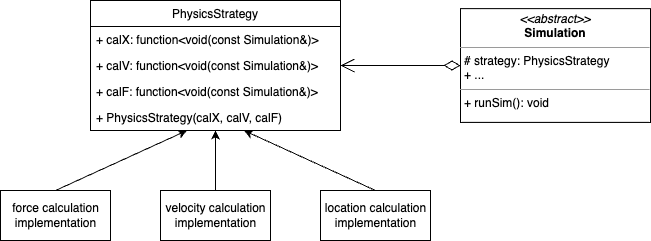
\includegraphics[width=\columnwidth]{../../../report/report1/res/strategy.png}
                \caption{UML-like diagram showing our implementation of the strategy pattern}
            \end{figure}
        \end{column}
    \end{columns}

    
\end{frame}

% Slides for mac_setup
\section{Force calculation}

\begin{frame}
    \frametitle{$F_{ij} = -F_{ji}$}
        \textbf{Task:} Implement Force calculation with the pairwise iterator

        \textbf{Solution:} Skip calculations due to $F_{ij} = -F_{ji}$
        \vspace{-15pt}
        \begin{equation}
            F_i = \sum_{j=1, j \neq i}^{\#particles} F_{i,j}
        \end{equation}
        \vspace{-15pt}
        \begin{align}
            F_{i,j} &= \frac{m_im_j}{(||x_i-x_j||_2)^3} (x_j - x_i) \\
                    &= \frac{m_jm_i}{(||x_j-x_i||_2)^3} \left(-1 \cdot \left(x_i - x_j\right)\right) = - F_{j,i}
        \end{align}
\end{frame}

\begin{frame}
    \frametitle{Force calculation}
    \begin{columns}
        \begin{column}{0.5\textwidth}
            \begin{table}[H]
                \begin{tabular}{|l|l|l|l|l|}
                \hline
                    & Time for $10^6$ iterations \\ \hline
                Naive & 31109ms                  \\ \hline
                V2    & 24881ms                  \\ \hline
                \end{tabular}
                \caption{Values measured for the two different force calculation strategies. Approx speedup of 1.25.}
                \label{tab:speedup}
            \end{table}
        \end{column}
        \begin{column}{0.5\textwidth}
            \begin{figure}[]
                \centering
                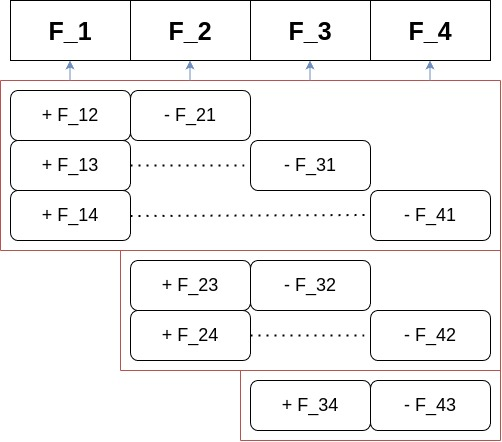
\includegraphics[width=\columnwidth]{ForceCalcFig.jpg}
                \caption{Pairwise Addition of Forces}
            \end{figure}
        \end{column}
    \end{columns}
\end{frame}

% Slides for References
\section{References}	
	\begin{thebibliography}
		\frame{
			\bibitem{StraPattern} https://refactoring.guru/design-patterns/strategy
		}
	\end{thebibliography}

\end{document}